\documentclass{beamer}
%\usepackage{amsfonts,amsmath,oldgerm}
\usetheme{sintef}
\usepackage{booktabs}
\usepackage{verbatim}
\usepackage{physics}
\usepackage{listings}
\usepackage{tikz} % Allows to draw custom shapes
\usepackage{tikzpagenodes}
\usepackage{appendixnumberbeamer}
\usepackage{pgfplots}
\pgfplotsset{compat=1.18}
\definecolor{listingkeywords}{rgb}{0.0, 0.5, 0.0}
\definecolor{listingidentifiers}{rgb}{0, 0, 0}
\definecolor{listingcomments}{rgb}{0.25, 0.5, 0.5}
\definecolor{listingstrings}{rgb}{0.73, 0.13, 0.13}
\definecolor{listingnumbers}{rgb}{0.25, 0.25, 0.25}
\lstdefinestyle{kaolst}{
	aboveskip=0.7\topskip,
	belowskip=0.1\topskip,
	basicstyle=\scriptsize\ttfamily,
	commentstyle=\color{listingcomments}\itshape,
	keywordstyle=\color{listingkeywords}\bfseries,
	numberstyle=\scriptsize\color{listingnumbers}\ttfamily,
	stringstyle=\color{listingstrings},
	identifierstyle=\color{listingidentifiers},
    morekeywords={for,set,end,each},
	breakatwhitespace=false,
	breaklines=true,
	captionpos=t,
	keepspaces=true,
	showspaces=false,
	showstringspaces=false,
	showtabs=false,
	numbers=none,
	numbersep=1em,
	%frame=lines,
	frame=none,
	framerule=.7pt,
	tabsize=4,
	defaultdialect=[LaTeX]Tex,
}
\lstdefinestyle{kaolstplain}{
	aboveskip=0.6\topskip,
	belowskip=-0.1\topskip,
	basicstyle=\scriptsize\ttfamily,
	commentstyle=\color{listingcomments}\itshape,
	keywordstyle=\color{listingkeywords}\bfseries,
	numberstyle=\scriptsize\color{listingnumbers}\ttfamily,
	stringstyle=\color{listingstrings},
	identifierstyle=\color{listingidentifiers},
	breakatwhitespace=false,
	breaklines=true,
	captionpos=t,
	keepspaces=true,
	showspaces=false,
	showstringspaces=false,
	showtabs=false,
	numbers=none,
	frame=none,
	tabsize=4,
	defaultdialect=[LaTeX]Tex,
}



\newcommand{\testcolor}[1]{\colorbox{#1}{\textcolor{#1}{test}}~\texttt{#1}}

%\usefonttheme[onlymath]{serif}

\titlebackground*{assets/background_old}

\newcommand{\hrefcol}[2]{\textcolor{cyan}{\href{#1}{#2}}}

\title{Neural Networks as Quantum States}
\subtitle{NNs in Quantum Many-Body Problems}
\course{Deep Learning con Applicazioni}
\author{\href{mailto:stefano.lonardoni1@studenti.unimi.it}{Stefano Lonardoni}}

\begin{document}
\maketitle

\begin{frame}{Introduction}
\framesubtitle{Neural Networks as Quantum States}
\begin{itemize}
	\item Quantum-many-body problems feature an exponential Hilbert-space growth
	\item Traditional variational ansätze reduce complexity sactificing correlation and entanglement
	\item Neural-network quantum states can offer expressivity with a compact set of parameters
\end{itemize}

\textbf{How Neural Networks can represent ground states for a many-body quantum system.}

\end{frame}

\begin{frame}{Restricted Boltzmann Machine}
\framesubtitle{Generative Model}
\begin{columns}
\begin{column}{0.68\textwidth}
\begin{itemize}
    \item Learns $p(\vec{x})$ of the input data $\vec{x}$
    \item Two layers: $N$ visible and $M$ hidden
    \item Trainable parameters $\mathcal{W}$: weights $W_{ij}$ and biases $b_i$, $c_j$
\end{itemize}
\end{column}
\begin{column}{0.3\textwidth}
\begin{center}
    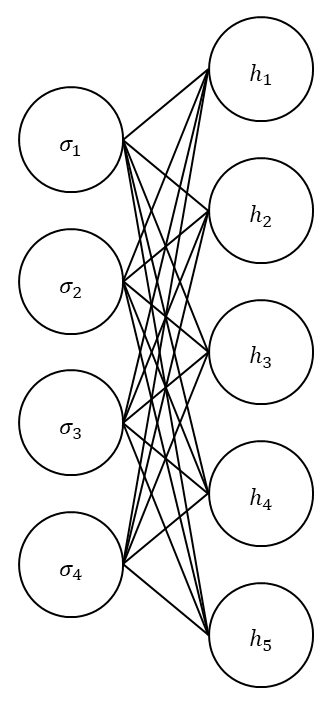
\includegraphics[height=\textheight]{images/rbm.png}
\end{center}
\end{column}
\end{columns}
\end{frame}

\begin{frame}{Restricted Boltzmann Machine}
\framesubtitle{Probability Distribution}
Internal Energy:
$$E(\vec{\sigma}, \vec{h}) = -\sum_{i} b_i v_i - \sum_{j} c_j h_j - \sum_{i,j} W_{ij} v_i h_j$$

Probability Distribution:
$$p(\vec{\sigma}, \vec{h}) = \frac{1}{Z} e^{-E(\vec{\sigma}, \vec{h})}$$

where $Z$ is the partition function:
$$Z = \sum_{\vec{\sigma}, \vec{h}} e^{-E(\vec{\sigma}, \vec{h})}$$
\end{frame}

\begin{frame}{Restricted Boltzmann Machine}
\framesubtitle{Application to Quantum States}
Considering a spin configuration $\vec{\sigma}$ and a set of parameters $\mathcal{W}$:
$$\psi\left( \vec{\sigma}, \mathcal{W} \right) = e^{\sum_{i} b_i \sigma_i + \sum_{j} c_j h_j + \sum_{i,j} W_{ij} \sigma_i h_j}$$

With no intra-layer connections:
$$\psi\left( \vec{\sigma}, \mathcal{W} \right) = e^{\sum_{i} b_i \sigma_i} \times \prod_{j=1}^{M} {\left[ c_j h_j + \sum_{i} W_{ij} \sigma_i h_j\right]}$$
\end{frame}

\begin{frame}{Training}
\framesubtitle{Reinforcement Learning}
\begin{columns}
\begin{column}{0.5\textwidth}
Minimize the energy expectation value:
$$E = \langle \hat{H} \rangle = \langle E_{\text{loc}} \rangle $$
\end{column}
\begin{column}{0.5\textwidth}    
where $E_{\text{loc}}$ is the local energy:
$$E_{\text{loc}}(\vec{\sigma}) = \frac{\hat{H} \psi\left( \vec{\sigma}, \mathcal{W} \right)}{\psi\left( \vec{\sigma}, \mathcal{W} \right)}$$
\end{column}
\end{columns}
\vskip1\baselineskip

The parameters $\mathcal{W}$ are optimized using a gradient descent method\footnote{Becca F, Sorella S. \textit{Quantum Monte Carlo Approaches for Correlated Systems}. Cambridge University Press; 2017}:
\begin{itemize}
	\item Variational Monte Carlo (VMC)
	\item Stochastic Reconfiguration (SR)
\end{itemize}

\end{frame}

\begin{frame}{Ground State Search}
\framesubtitle{Variational Monte Carlo}
We can compute the gradients:
\begin{equation*}
\begin{aligned}
    \nabla_{\mathcal{W}} E &= \nabla_{\mathcal{W}} \langle E_{\text{loc}} \rangle \\
    &= \langle E_{\text{loc}} \nabla_{\mathcal{W}} log(p_{\psi}) \rangle \\
    &= 2 \mathfrak{R} \left[ \langle E_{\text{loc}} \nabla_{\mathcal{W}} log(\psi) \rangle - \langle E_{\text{loc}} \rangle \langle \nabla_{\mathcal{W}} log(\psi) \rangle \right]
\end{aligned}
\end{equation*}
And consequently update the parameters:
$$\mathcal{W}^{'} = \mathcal{W} - \eta \nabla_{\mathcal{W}} E$$
\end{frame}

\begin{frame}{Ground State Search}
\framesubtitle{Stochastic Reconfiguration}
Parameters evolution in the variational space:
$$\mathcal{W}\left( p + 1\right) = \mathcal{W}\left( p \right) - \mathbf{S}^{-1} \vec{F}$$
where $\mathbf{S}^{-1}$ is the pseudo-inverse of the covariance matrix:
$$\mathbf{S}_{ij} = \langle O_i^{*} O_j \rangle - \langle O_i^{*} \rangle \langle O_j \rangle$$
and $\vec{F}$ is the gradient of the energy:
$$F_i = \langle O_i^{*} E_{\text{loc}} \rangle - \langle O_i^{*} \rangle \langle E_{\text{loc}} \rangle$$
where $O_i$ are the local operators defined as:
$$O_i = \frac{\partial log\left(\psi\left( \vec{\sigma}, \mathcal{W} \right)\right)}{\partial W_{ij}}$$

\end{frame}

\begin{chapter}[assets/background_negative]{}{Code Implementation}
\begin{itemize}
    \item RBM
    \item Sampler
    \item Hamiltonian
    \item Optimizers
\end{itemize}
\end{chapter}

\begin{frame}[fragile]{Code Implementation}
\framesubtitle{RBM}

Custom \lstinline[style=kaolstplain]|tf.module| implementing the RBM.
\vskip1\baselineskip

Weights and biases are initialized randomly as complex values:
\begin{lstlisting}[language=Python, style=kaolstplain]
self.W = tf.Variable(
	tf.random.normal([self.N_visible, self.N_hidden], dtype=tf.complex64)
)
self.b = tf.Variable(tf.random.normal([self.N_visible], dtype=tf.complex64))
self.c = tf.Variable(tf.random.normal([self.N_hidden], dtype=tf.complex64))
\end{lstlisting}
\begin{center}
    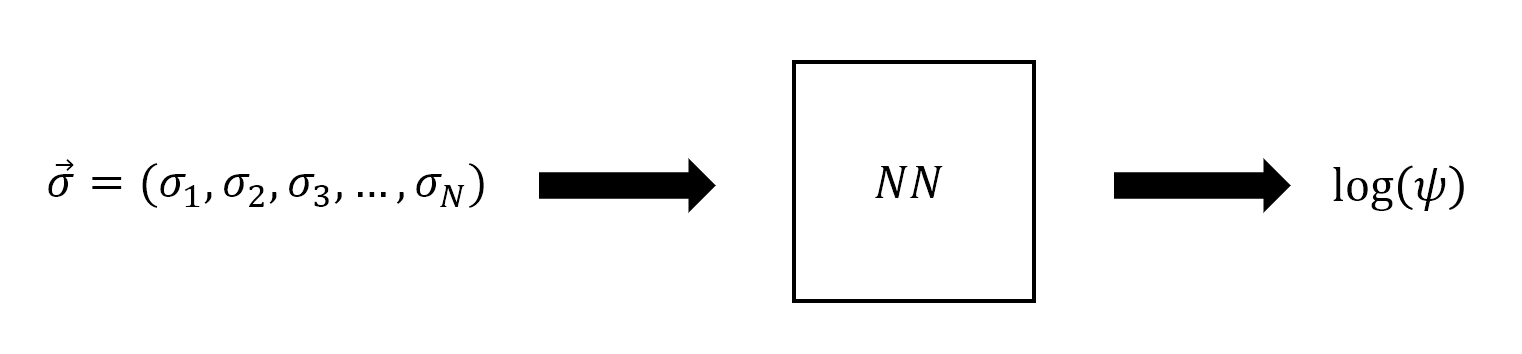
\includegraphics[height=3cm]{images/rbm_usage.png}
\end{center}

\end{frame}

\begin{frame}[fragile]{Code Implementation}
\framesubtitle{RBM - Logarithm of the Wave Function}
Provides method to compute the logarithm of the wave function:
\begin{lstlisting}[language=Python, style=kaolstplain]
def log_psi(self, samples):
    casted_samples = 2.0 * tf.cast(samples, tf.complex64) - tf.ones_like(samples, dtype=tf.complex64)
    sum_visible = tf.reduce_sum(self.a * casted_samples, axis=1)
    w_h = self.b + tf.matmul(casted_samples, self.W)
    sum_hidden = tf.reduce_sum(tf.math.log(2.0 * (tf.math.cosh(self.b + tf.matmul(casted_samples, self.W)))), axis=1)
    return sum_visible + sum_hidden
\end{lstlisting}
\end{frame}


\begin{frame}[fragile]{Code Implementation}
\framesubtitle{Sampler}

Samples configurations from the RBM.

\begin{itemize}
    \item \textbf{Metropolis-Hastings} Random Walk using TensorFlow Probability
    \item \textbf{Gibbs sampling} Double-step method to sample visible and hidden variables
\end{itemize}

Provides batches of configurations. Example:
\begin{lstlisting}[language=Python, style=kaolstplain]
>>> sam.sample(rbm)
<tf.Tensor: shape=(5, 4), dtype=float32, numpy=
array([[0., 0., 0., 0.],
       [1., 1., 1., 0.],
       [0., 0., 1., 0.],
       [0., 0., 0., 0.],
       [0., 0., 0., 1.]], dtype=float32)>
\end{lstlisting}

\end{frame}

\begin{frame}{Code Implementation}
\framesubtitle{Hamiltonian}
Class representing the Hamiltonian of the system.
\begin{itemize}
    \item \textbf{Ising1D} Ising model in 1D
    \item \textbf{TFIH} Transverse Field Ising Hamiltonian
\end{itemize}

Provides methods to compute the local energy from a batch of configurations.

\end{frame}

\begin{frame}[fragile]{Code Implementation}
\framesubtitle{Optimizers}
Both VMC and SR optimizers leverage \lstinline[style=kaolstplain]|tf.GradientTape| to compute gradients.
\begin{lstlisting}[language=Python, style=kaolstplain]
with tf.GradientTape() as tape:
	log_psi = self.wave_function.log_psi(samples)

grad_log_psi = tape.jacobian(log_psi, self.wave_function.trainable_variables)
\end{lstlisting}
\vskip1\baselineskip

Both methods update the parameters of the wave function in the same way:
\begin{lstlisting}[language=Python, style=kaolstplain]
for grad_val, var in grads_vars:
	var.assign_sub(self.learning_rate * grad_val)
\end{lstlisting}
\end{frame}

\begin{frame}[fragile]{Code Implementation}
\framesubtitle{Optimizers - VMC}
The VMC approach computes the variational increments as follows:
\begin{lstlisting}[language=Python, style=kaolstplain]
mean_energy = tf.reduce_mean(local_energies)
for grad_i in grad_log_psi:
	if grad_i is not None:
		expand_shape = tf.concat([[tf.shape(local_energies)[0]], tf.ones(tf.rank(grad_i) - 1, dtype=tf.int32)], axis=0)
		e_loc_expanded = tf.reshape(local_energies, expand_shape)
		loc_grad = e_loc_expanded * grad_i
		grad_energy = tf.reduce_mean(loc_grad, axis=0)
		grad_log_psi_mean = tf.reduce_mean(grad_i, axis=0)

		vmc_grad = 2.0 * tf.math.real(grad_energy - mean_energy * grad_log_psi_mean)
		vmc_grad = tf.cast(vmc_grad, tf.complex64)  # Ensure dtype matches variable
		gradients.append(vmc_grad)
	else:
		gradients.append(None)
\end{lstlisting}
\end{frame}

\begin{frame}[fragile]{Code Implementation}
\framesubtitle{Optimizers - Stochastic Reconfiguration}
The SR approach computes the variational increments as follows:
\begin{lstlisting}[language=Python, style=kaolstplain]
O = tf.concat(flat_grads, axis=1)
O_mean = tf.reduce_mean(O, axis=0)
# compute covariance matrix / QGT
O_O = tf.matmul(O_mean, O_mean, transpose_a=True)
norm = tf.cast(n_samples, O_centered.dtype)
S = O_O / norm
# compute force vector
mean_energy = tf.reduce_mean(local_energies)
F_vec = (
	tf.reduce_mean(local_energies[:, None] * O, axis=0) - mean_energy * O_mean
)
# solve for delta
P = tf.shape(S)[0]
S_reg = S + self.epsilon * tf.eye(P, dtype=S.dtype)
gradients = tf.linalg.solve(S_reg, tf.expand_dims(F_vec, 1))
\end{lstlisting}
\end{frame}

\begin{chapter}[assets/background_negative]{}{Results}
\end{chapter}

\begin{frame}{Results}
\framesubtitle{1D Ising Model - 8 spins}
\end{frame}

\begin{frame}{Results}
\framesubtitle{TFIH - 8 spins}
\end{frame}

\begin{frame}{Further Work}
\framesubtitle{Optimization and Extensions}
\begin{columns}
\begin{column}{0.5\textwidth}
\begin{itemize}
	\item Extend to 2D systems
	\item Other neural networks (FFNN, CNN)
	\item Unitary (and non) dynamics
\end{itemize}
\end{column}
\begin{column}{0.5\textwidth}
\begin{itemize}
	\item Efficient SR update (single parameter updates)
	\item Change tensor framework (JAX, ...)
\end{itemize}
\end{column}
\end{columns}
\end{frame}

\begin{frame}{Other Works}
\begin{columns}
\begin{column}{0.6\textwidth}
\textbf{NetKet}: The Machine-Learning toolbox for Quantum Physics
\end{column}
\begin{column}{0.3\textwidth}

\includegraphics[width=\textwidth]{images/netket.png}
\end{column}
\end{columns}
\end{frame}

\begin{frame}{References}

\end{frame}

\backmatter

\appendix


\begin{chapter}[assets/background_negative]{}{Appendix}
\end{chapter}

\begin{frame}{Appendix}
\framesubtitle{Probabilities for the RBM}
Conditional probabilities for visible and hidden
\end{frame}

\begin{frame}{Appendix}
\framesubtitle{Local operators for the RBM}
Explicit form of the partial derivatives of $log\left(\psi\right)$


\end{frame}

\begin{frame}{Appendix}
\framesubtitle{Metropolis-Hastings and MCMC sampling}
\end{frame}

\begin{frame}{Appendix}
\framesubtitle{Gibbs sampling}
\end{frame}

\begin{frame}{Appendix}
\framesubtitle{1D Ising Model}
\end{frame}

\begin{frame}{Appendix}
\framesubtitle{Transverse Field Ising Hamiltonian}
\end{frame}

\end{document}
